\section{Replace}
\begin{enumerate}
\item IDA打开很容易找到WinMain函数,直接分析窗口函数DialogFunc\\
	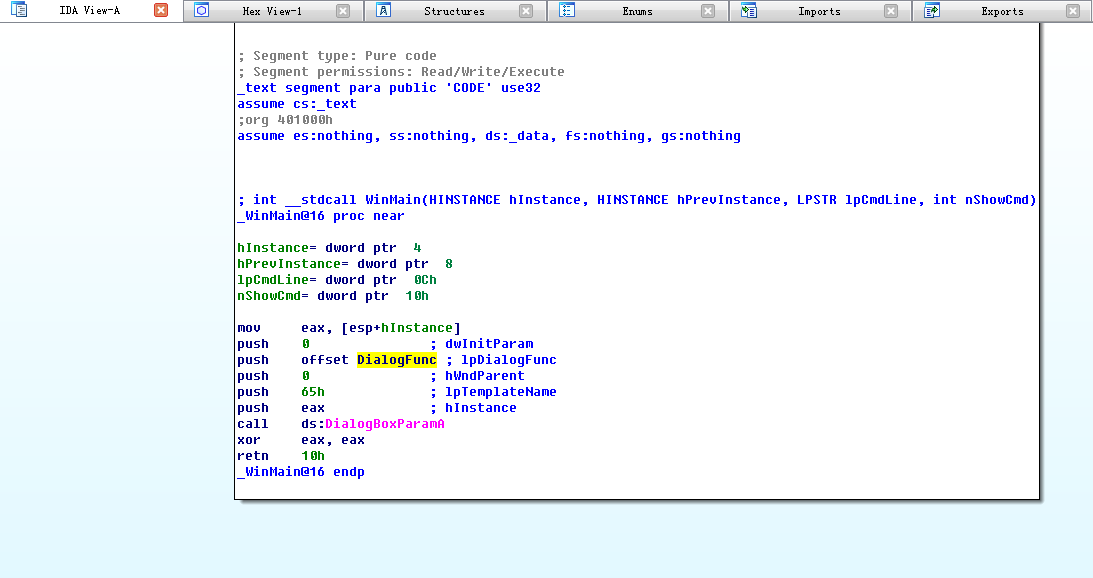
\includegraphics[width=10cm]{replace-winmain} \\
\item 
	\begin{enumerate}
	\item 找到函数调用GetDlgItemInt,获取输入,存放在\lstinline$dword_4084D0$\\
	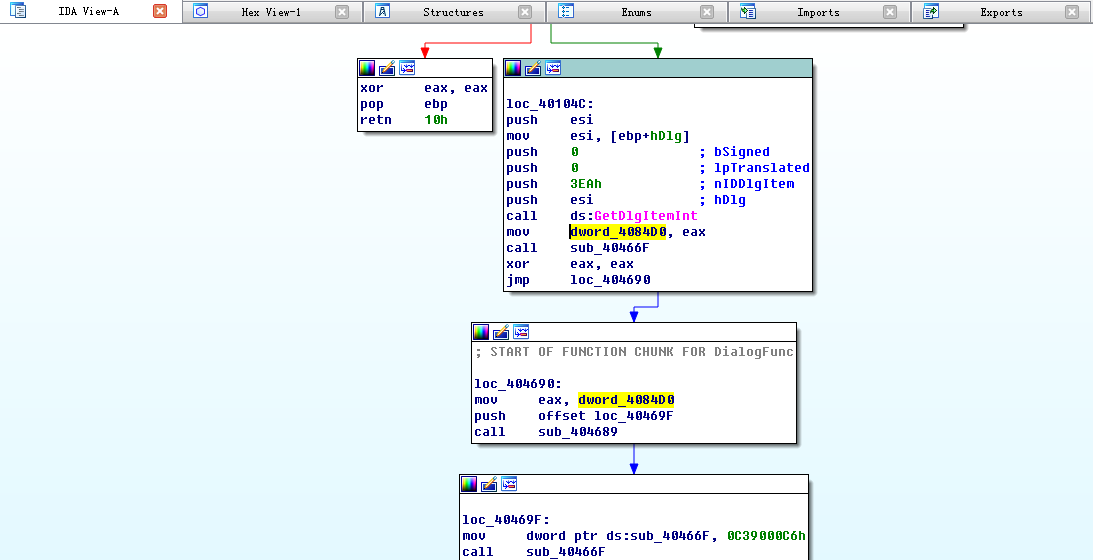
\includegraphics[width=10cm]{replace-getdlgitemint} \\
	\item 关键函数\lstinline$sub_40466F$调用了三次,\\
	\item 第一次调用函数\lstinline$sub_40466F$:\\
	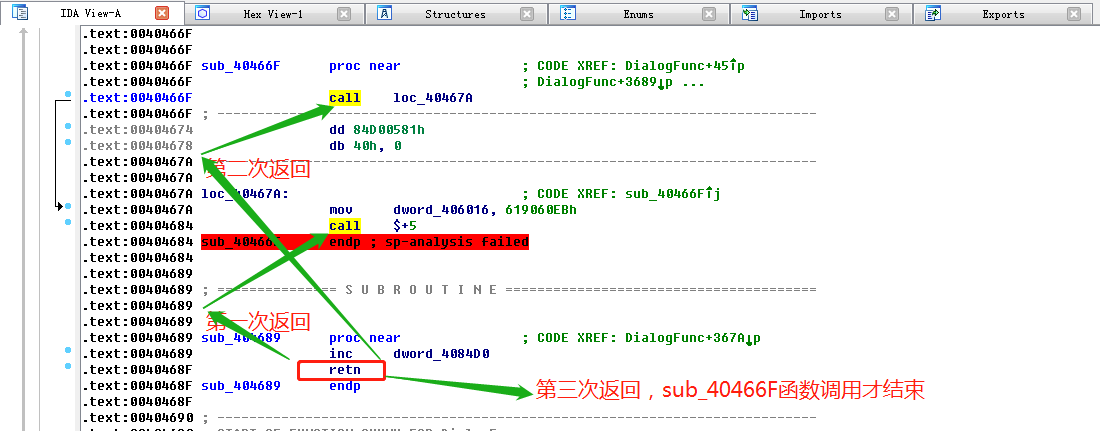
\includegraphics[width=10cm]{replace-func1} \\
	针对\lstinline$dword_4084D0$的操作:
	\begin{lstlisting}
	inc     dword_4084D0
	inc     dword_4084D0
	\end{lstlisting}
	第二次返回之后:\lstinline$call loc_40467A$之后的语句转换为代码(.text:00404674地址处,按C转换为代码)
	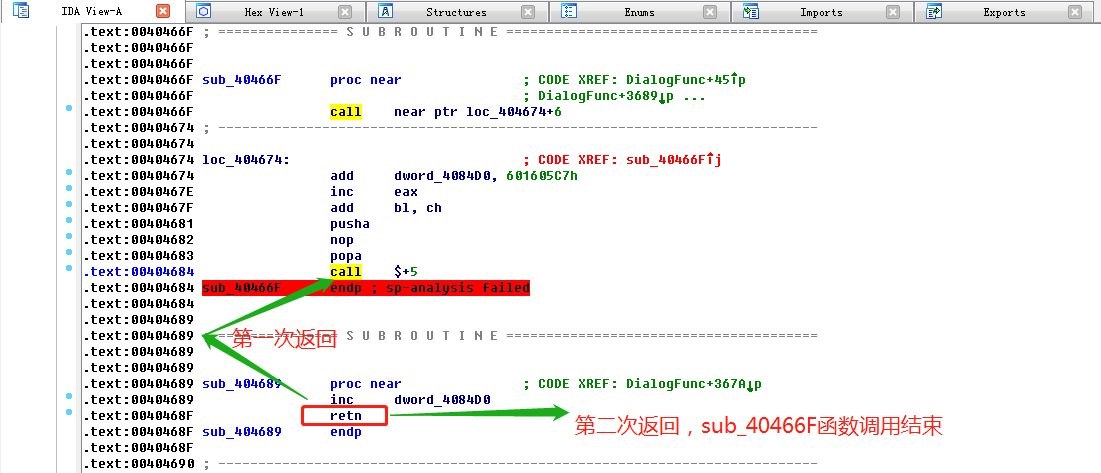
\includegraphics[width=10cm]{replace-func2} \\
	针对\lstinline$dword_4084D0$的操作:
	\begin{lstlisting}
	add     dword_4084D0, 601605C7h
	inc     dword_4084D0
	inc     dword_4084D0
	\end{lstlisting}
	\item 第二次调用\lstinline$sub_40466F$函数时,函数已经被修改:\\
	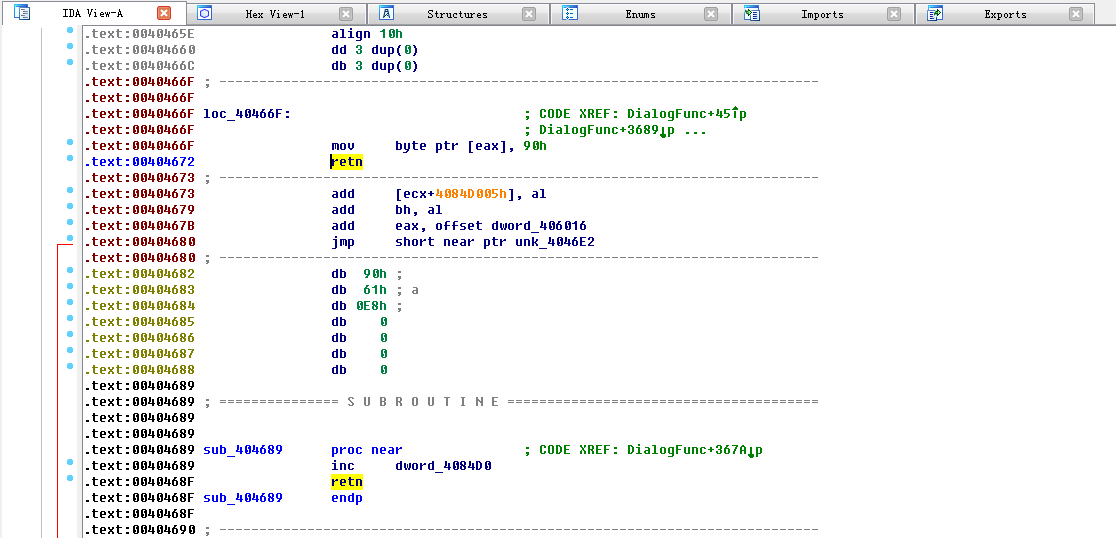
\includegraphics[width=10cm]{replace-func3} \\
	\begin{lstlisting}
	mov	byte ptr [eax], 90h
	\end{lstlisting}
	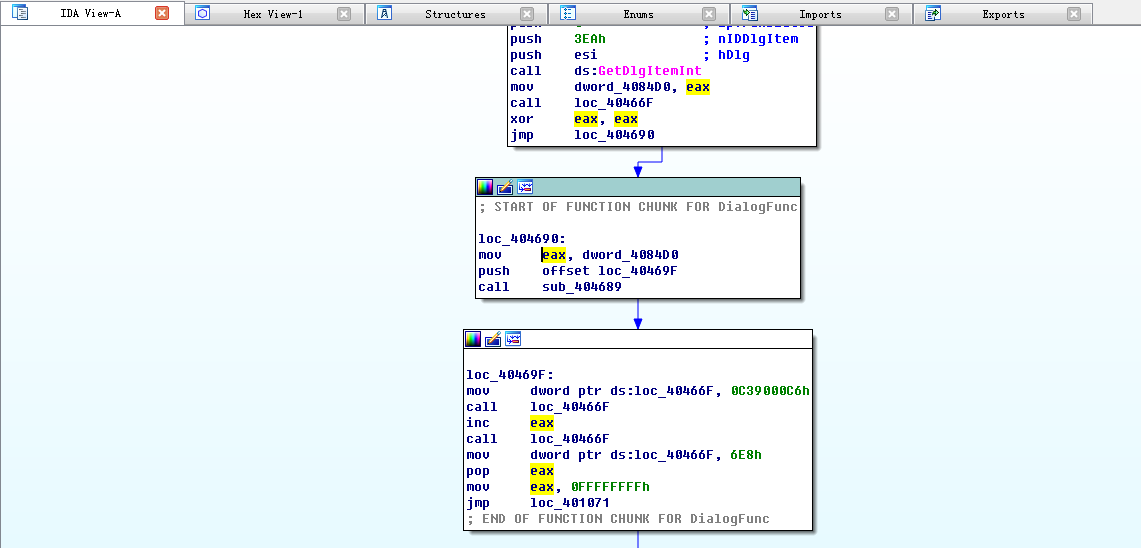
\includegraphics[width=10cm]{replace-eax} \\
	\item 紧接着eax加1,第三次调用\lstinline$sub_40466F$函数,关键就在这里了,好久之后终于悟到\\
	\end{enumerate} 
\item 
	 显示字符串“\lstinline$Correct!$”分支无路径可以到达,只有修改代码:\\
	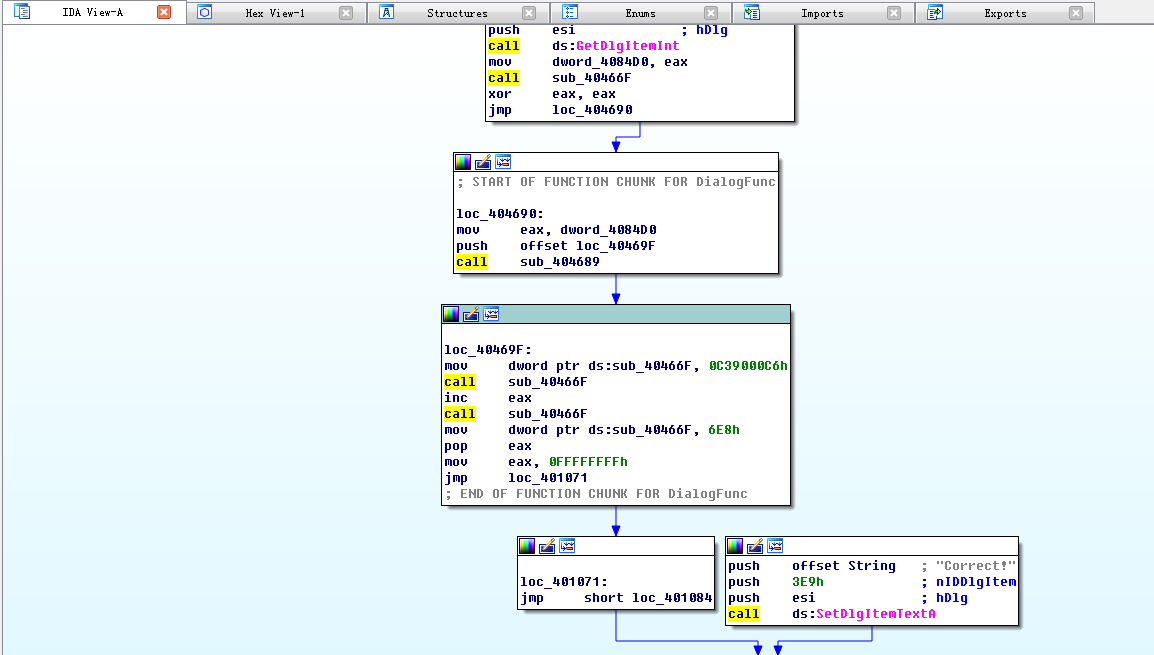
\includegraphics[width=10cm]{replace-overview} \\
	 分析显示字符串“\lstinline$Correct!$”分支代码:\\
	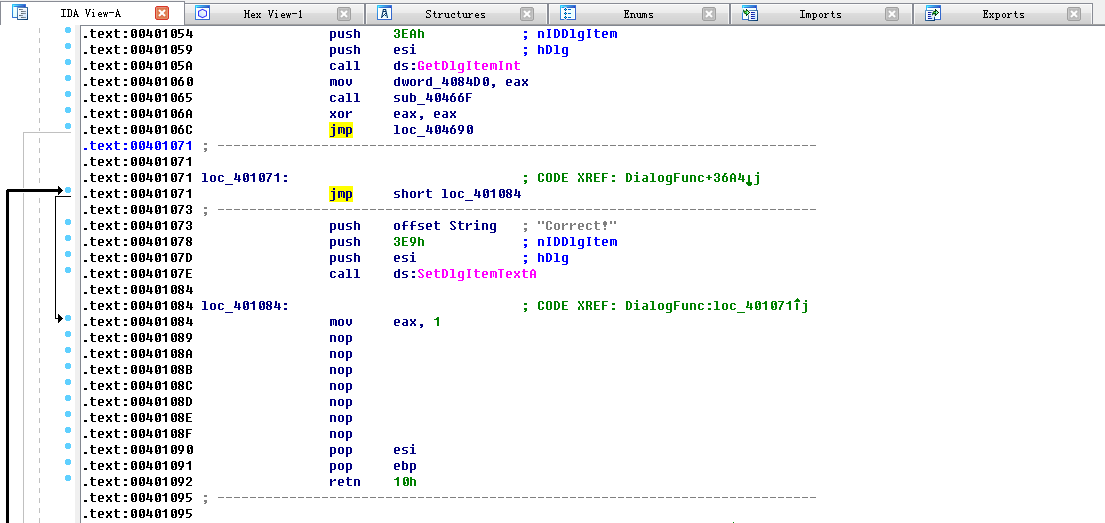
\includegraphics[width=10cm]{replace-jump} \\
	分析整理:第一次调用函数\lstinline$sub_40466F$\\
	\begin{lstlisting}
	inc     dword_4084D0
	inc     dword_4084D0
	add     dword_4084D0, 601605C7h
	inc     dword_4084D0
	inc     dword_4084D0
	\end{lstlisting}
	\lstinline$dword_4084D0$值赋给eax, (之后调用的\lstinline$sub_404689$函数,\\
	也对\lstinline$dword_4084D0$执行了加1操作,但此时\lstinline$dword_4084D0$的值已经不重要了)\\
	连续两次调用函数\lstinline$sub_40466F$,90h为nop的操作码,\\
	即将eax指向的两个连续字节修改为nop、nop,如果eax值为.text:00401071,\\
	判定正确之前的jmp被修改为nop、nop了,分支就有机会执行了\\
	输入 + 4 + 0x601605C7 - 0xFFFFFFFF - 1 = 0x401071 \\
	( - 0xFFFFFFFF - 1是因为0x401071 < 0x601605C7,加法需要溢出)\\
	整理一下:\\
	输入 = 0x401071 +1 + 0xFFFFFFFF - 0x601605C7 - 4 \\
	shell(cmd)中执行:\\ 
	perl -e "print 0x401071+1+0xFFFFFFFF-4-0x601605C7" \\
	获取flag: "2687109798"
\end{enumerate}